\documentclass[aps,prb,onecolumn,notitlepage,showpacs,floatfix,superscriptaddress]{revtex4-1}
\usepackage{dcolumn}
\usepackage{tabularx}
\usepackage{bm}
\usepackage{soul}
\usepackage{amsmath,amssymb,graphicx}
\usepackage[colorlinks=true,citecolor=blue,urlcolor=blue,linkcolor=blue]{hyperref}
\usepackage{environ}

\NewEnviron{eqnsplit}{%
\begin{equation}
\begin{split}
  \BODY
\end{split}
\end{equation}
}

\newcommand{\mrm}[1]{\mathrm{#1}}
\newcommand{\ang}{\mathrm{\AA}}

\bibliographystyle{apsrev4-1}

%%%%%%%%%%%%%%%%%%%%%%%%%%%%%%%%%%%%%%%%%%%%%%%%
\begin{document}

\title{Kramers Kronig Relations}

\author{Avinash Rustagi}
\email{arustag@ncsu.edu}
\affiliation{Department of Physics, North Carolina State University, Raleigh, NC 27695}
%
\date{\today}
%%%%%%%%%%%%%%%%%%%%%%%%%%%%%%%%%%%%%%%%%%%%%%%%

\maketitle
%
\section{Retarded}
Causality means that the cause precedes the effects. A simple model case is the retarded Green function
\begin{equation}
G^R_k(t-t')=-i\theta(t-t') \langle \{ c_k(t),c_k^\dagger(t')\}\rangle = -i\theta(t-t') e^{-i\varepsilon_k (t-t')}
\end{equation}
In Fourier space
\begin{equation}
\begin{split}
G^R(\omega) &= \int_{-\infty}^\infty d(t-t') \, G^R_k(t-t') e^{i \omega (t-t')} \\
&= -i\int_{0}^\infty d(t-t') \, e^{i (\omega-\varepsilon_k) (t-t')} 
\end{split}
\end{equation}
To make the integral converge, we can introduce a small positive infinitesimal factor $\delta$
\begin{equation}
\begin{split}
G^R(\omega) &= -i\int_{0}^\infty d(t-t') \, e^{i (\omega-\varepsilon_k) (t-t')} e^{-\delta(t-t')} \\
 &= -i\int_{0}^\infty d(t-t') \, e^{i (\omega-\varepsilon_k+i\delta) (t-t')} \\
 &= \dfrac{1}{\omega-\varepsilon_k+i\delta}
\end{split}
\end{equation}
The retarded Green function has poles in the lower half of the complex plane and is analytic in the upper half. \\

Consider a function $\chi_R$ with a pole on the real axis and is analytic in the upper half of the complex plane. Then by Cauchy's theorem
\begin{equation}
\oint_C dz\, \dfrac{\chi_R(z)}{z-\omega_0} =0
\end{equation}
where the contour $C$ does not include the singularity.
\begin{figure}[hbtp]
\centering
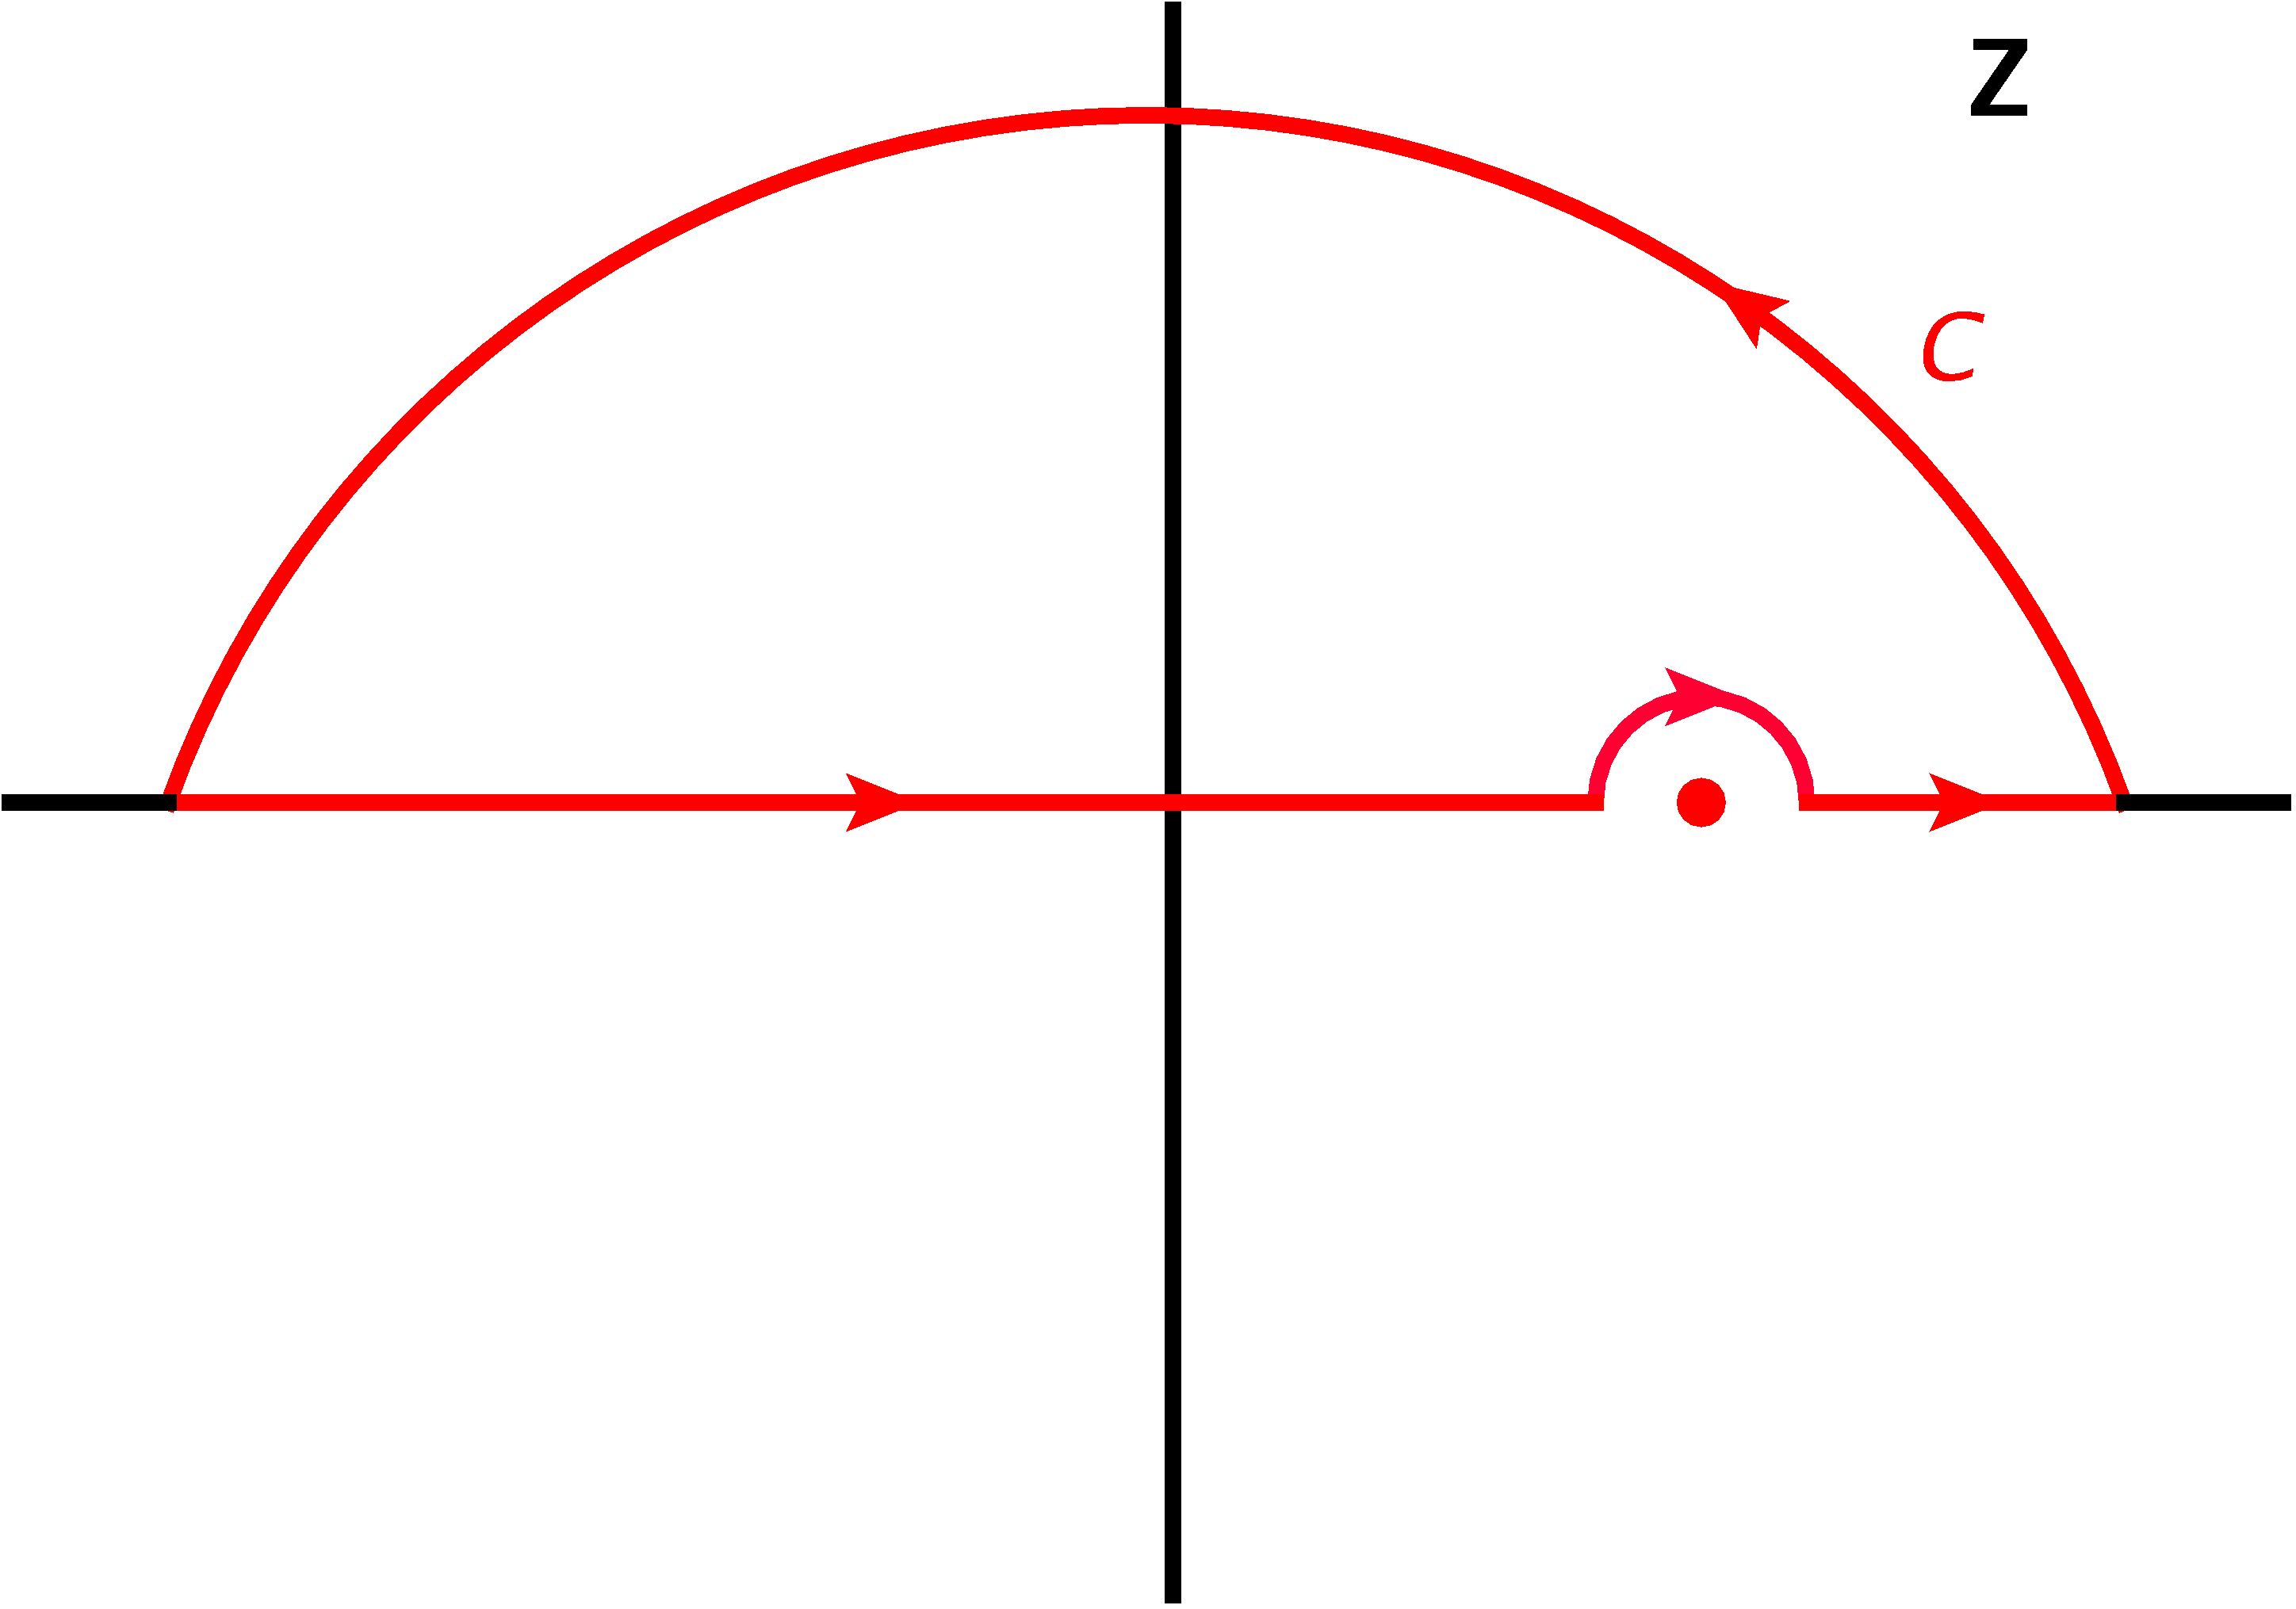
\includegraphics[scale=0.07]{retarded.png}
\caption{Contour for Retarded function that is analytic in the entire upper half plane.}
\end{figure}
\begin{equation}
\begin{split}
&\oint_C dz\, \dfrac{\chi_R(z)}{z-\omega_0} =0 \\
&\lim_{\epsilon \rightarrow 0}\int_{-\infty}^{\omega_0-\epsilon} d\omega \, \dfrac{\chi_R(\omega)}{\omega-\omega_0} + \lim_{\epsilon \rightarrow 0} \int_{\omega_0-\epsilon}^\infty d\omega \, \dfrac{\chi_R(\omega)}{\omega-\omega_0} -i \pi \chi_R(\omega_0)=0 \\
\Rightarrow \quad & \mathcal{P}\int_{-\infty}^\infty d\omega \, \dfrac{\chi_R(\omega)}{\omega-\omega_0} = i\pi \chi_R (\omega_0)
\end{split}
\end{equation}
The function $\chi_R = \chi_R' +i \chi_R''$ is complex. Thus comparing the real and imaginary parts
\begin{equation}
\begin{split} 
 \chi_R' (\omega_0) &=\dfrac{1}{\pi} \mathcal{P}\int_{-\infty}^\infty d\omega \, \dfrac{\chi_R''(\omega)}{\omega-\omega_0} \\
  \chi_R'' (\omega_0) &= -\dfrac{1}{\pi}\mathcal{P}\int_{-\infty}^\infty d\omega \, \dfrac{\chi_R'(\omega)}{\omega-\omega_0} 
\end{split}
\end{equation}

\section{Advanced}
Anti-Causality means that the effect precedes the cause. A simple model case is the advanced Green function
\begin{equation}
G^A_k(t-t')=i\theta(t'-t) \langle \{ c_k(t),c_k^\dagger(t')\}\rangle = i\theta(t'-t) e^{-i\varepsilon_k (t-t')}
\end{equation}
In Fourier space
\begin{equation}
\begin{split}
G^A(\omega) &= \int_{-\infty}^\infty d(t-t') \, G^A_k(t-t') e^{i \omega (t-t')} \\
&= i\int_{-\infty}^0 d(t-t') \, e^{i (\omega-\varepsilon_k) (t-t')} 
\end{split}
\end{equation}
To make the integral converge, we can introduce a small positive infinitesimal factor $\delta$
\begin{equation}
\begin{split}
G^A(\omega) &= i\int_{-\infty}^0 d(t-t') \, e^{i (\omega-\varepsilon_k) (t-t')} e^{\delta(t-t')} \\
 &= i\int_{-\infty}^0 d(t-t') \, e^{i (\omega-\varepsilon_k-i\delta) (t-t')} \\
 &= \dfrac{1}{\omega-\varepsilon_k-i\delta}
\end{split}
\end{equation}
The advanced Green function has poles in the upper half of the complex plane and is analytic in the lower half. \\
\begin{figure}[hbtp]
\centering
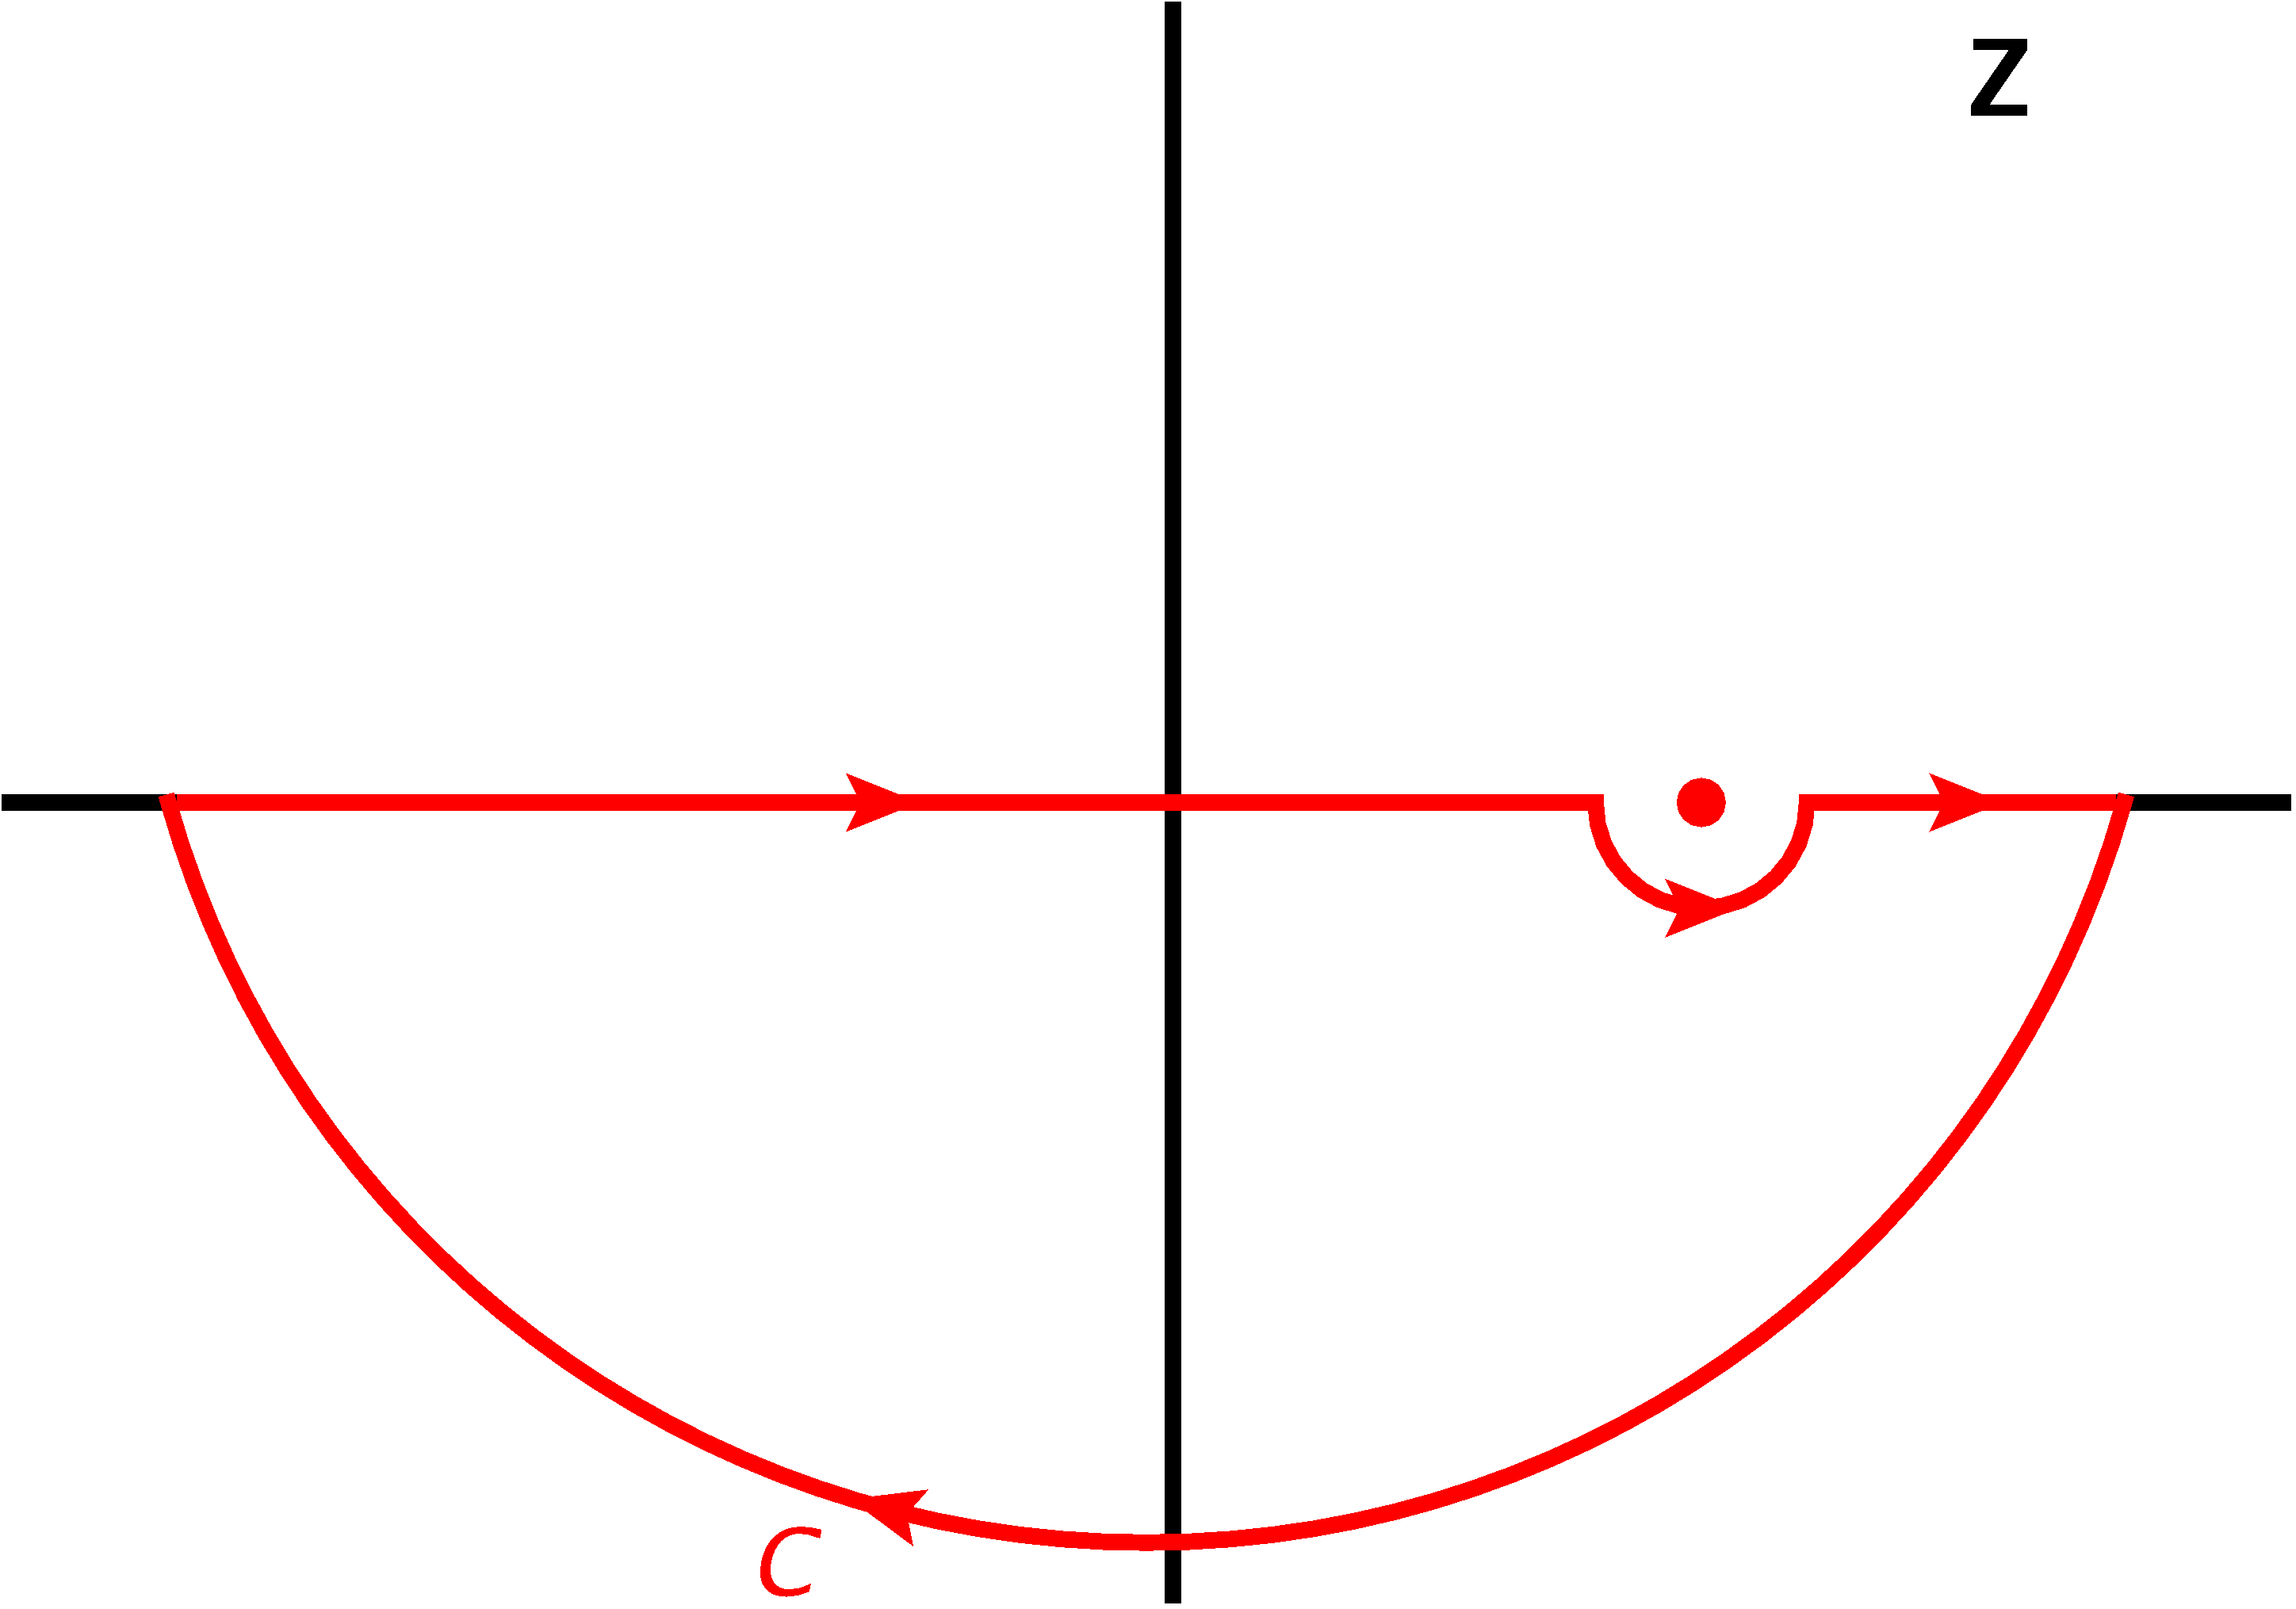
\includegraphics[scale=0.07]{advanced.png}
\caption{Contour for Advanced function that is analytic in the entire lower half plane.}
\end{figure}
Consider a function $\chi_A$ with a pole on the real axis and is analytic in the lower half of the complex plane. Then by Cauchy's theorem
\begin{equation}
\oint_C dz\, \dfrac{\chi_A(z)}{z-\omega_0} =0
\end{equation}
where the contour $C$ does not include the singularity.
\begin{equation}
\begin{split}
&\oint_C dz\, \dfrac{\chi_A(z)}{z-\omega_0} =0 \\
&\lim_{\epsilon \rightarrow 0}\int_{-\infty}^{\omega_0-\epsilon} d\omega \, \dfrac{\chi_A(\omega)}{\omega-\omega_0} + \lim_{\epsilon \rightarrow 0} \int_{\omega_0-\epsilon}^\infty d\omega \, \dfrac{\chi_A(\omega)}{\omega-\omega_0} +i \pi \chi_A(\omega_0)=0 \\
\Rightarrow \quad & \mathcal{P}\int_{-\infty}^\infty d\omega \, \dfrac{\chi_A(\omega)}{\omega-\omega_0} = -i\pi \chi_A (\omega_0)
\end{split}
\end{equation}
The function $\chi_A = \chi_A' +i \chi_A''$ is complex. Thus comparing the real and imaginary parts
\begin{equation}
\begin{split} 
 \chi_A' (\omega_0) &=-\dfrac{1}{\pi} \mathcal{P}\int_{-\infty}^\infty d\omega \, \dfrac{\chi_A''(\omega)}{\omega-\omega_0} \\
  \chi_A'' (\omega_0) &= \dfrac{1}{\pi}\mathcal{P}\int_{-\infty}^\infty d\omega \, \dfrac{\chi_A'(\omega)}{\omega-\omega_0} 
\end{split}
\end{equation}

\end{document}